\subsection{Inner Detector Tracks}
\label{sec:idtracks}
\par Track reconstruction in the Inner Detector begins with the identification 
of {\it spacepoints}. These are spatial points per sensor that were hit by a charged  
ionizing particle. These hits are collected in the Pixel Detector and the Semi-Conductor 
Tracker (SCT) which are collectively known as Silicon Detectors. In the Pixel Detector a hit on a 
pixel provides a 2-dimensional spacepoint, while a hit on an SCT sensor provides a 1-dimensional 
spacepoint; the other dimension in the SCT is provided by another sensor glued back-to-back and 
at an angle to the aforementioned sensor, as described in Section~\ref{sec:ID}.
The spacepoints in the silicon detectors are fitted using the Kalman Fitter~\cite{citeulike:347166} 
which adds spacepoints to the fit recursively, making it convenient for online real 
time processing.   

\par The result of each fit is characterized by a score that is calculated from the 
quality of the reconstructed track and the $\chi^2$ value of the fit. Track quality 
is determined by the number and {\it type} of hits that it constitutes. The type of a hit 
refers to its location in the ID: Pixel Detector hits are given more weight than
 SCT hits. At this stage of reconstruction different tracks may 
share hits, leading to ambiguities. These ambiguities in hits are resolved by giving 
preference to a track with the highest score, refitting the other tracks without the ambigous 
hits, and re-evaluating the scores. This process is repeated until all ambiguities are resolved. 

\par Hits from the Transition Radiation Tracker (TRT) are also fitted using the Kalman Fitter 
to tracks reconstructed from the silicon detectors. If the score of the resultant track 
improves the score of the silicon track, the TRT component is added. Otherwise it is 
reconstructed as an independent track. Tracks from the TRT are sometimes used as seed for 
track reconstruction, but tracks used in this thesis are reconstructed with hits from the 
silicon detector as seeds.  

\par Reconstructed tracks are parametrized by the point of their 
closest approach to either the beam-line or the interaction point (IP). The beam-line or 
the IP is known as the {\it perigee}. The perigee is in turn parametrized by {\it perigee parameters}. 
 Using the beam-line as reference is a more useful parametrization because the beam-line does not always 
align perfectly with the $z$-axis. The most common perigee parameters are $d_0$ and $z_0$, and their 
definitions are illustrated in Figure~\ref{fig:impctPV}. $d_0$ is the signed distance of the track's 
closest point to the $z$-axis, and $z_0$ is its $z$-coordinate. Other parameters defined at the perigee are the charge-momentum 
ratio, the angle with the $x$-axis in the $xy$ plane, and the angle with the $z$-axis 
in the $rz$ plane. Figure~\ref{fig:impctPV} illustrates most of them.  
 
\begin{figure}[!h]
\centering
   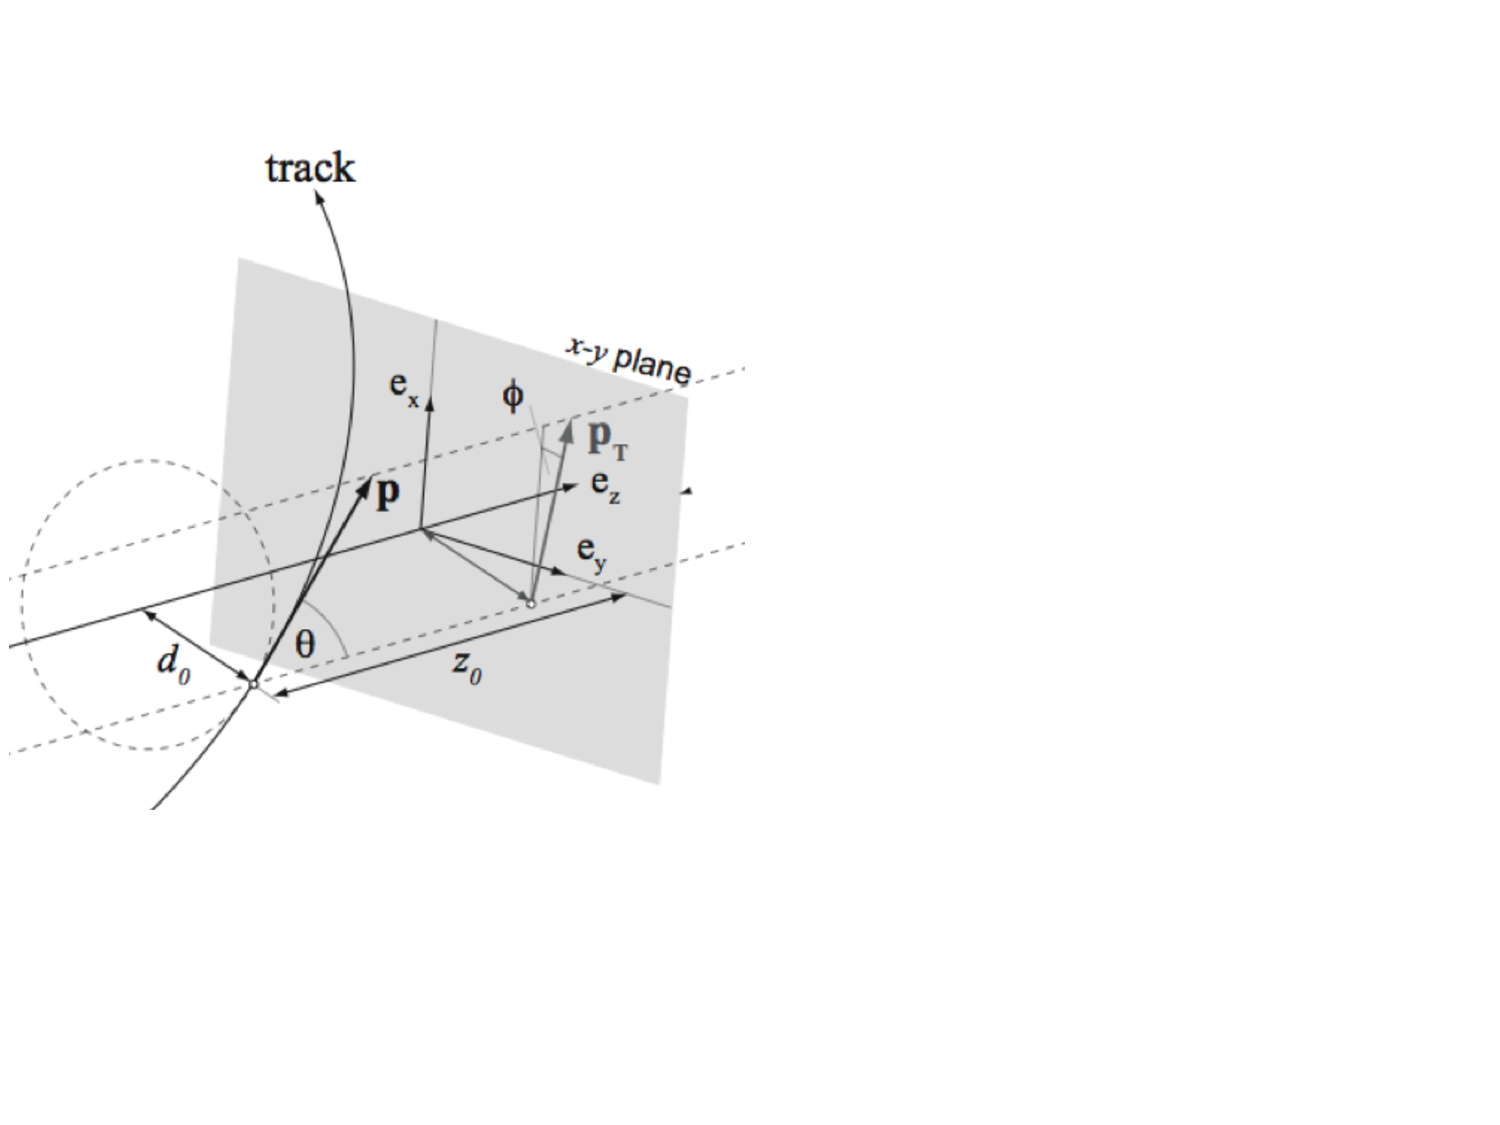
\includegraphics[width=0.8\textwidth]{figures/trkImp.pdf}
	\caption{Illustration of perigee parameters. The most common of these are $d_0$ and $z_0$. The perigee 
may be defined relative to either the beam-line or the interaction point. The analysis in Chapter~\ref{exclH} 
utilizes this choice. Illustration taken from Ref~\cite{ATLAS:trkImp}}
	\label{fig:impctPV}
\end{figure}

\par If a group of tracks reconstructed in the ID are extrapolated to a single spatial 
point in the ID, that point is reconstructed as a vertex. A vertex essentially represents 
a point where a particle, or particles, decay or split into secondary particles that leave 
tracks in the ID. The vertex with the highest sum of track transverse momentum, \pt, is labeled the 
primary vertex (PV). This is the vertex at which the hard scatter occurs. Since the PV does not 
always coincide with the IP, track perigees are usually measured relative to the PV.  

\subsection{Muon Spectrometer Tracks}
\par Seeds for MS track reconstruction are extracted from the precision 
sub-detectors: Cathode Strip Chambers (CSCs) and Monitored Drift Tubes (MTDs).
From MDTs drift circles are processed, and from CSCs {\it clusters} are built.
Signals from drift circles and clusters are used as inputs to pattern recognition algorithms 
to form {\it segments}, which are combined and fitted to form the reconstructed track. 

\par Clusters in the CSCs are muon hits in each chamber that give a 1-dimensional measurement of 
position. Since CSCs are mounted on wheels in the end-caps and are segmented in $\phi$, separate 
$\phi$ and $\eta$ clusters are obtained. A set of clusters is fitted using the Hough transform 
method~\cite{Kiryati:1991:PHT:104022.104026}, which is more suited to fitting non-linear tracks than the Kalman Fitter, to form 
separate $\eta$ and $\phi$ segments. Combining the two gives a 2-dimensional position and a 
direction to each cluster.  

\par Segments in the MDTs are reconstructed from fitting drift circles measured from 
drift tubes in two neighboring stations. Two outer MDT hits are picked as seeds and straight 
lines are fitted between them, accounting for hits in the middle layer. With a minimum of 3 hits 
required to form a segment, the fit with the 
highest number of hits is picked. The quality of an individual hit in an MDT is best described by Figure~\ref{fig:mstrackQ}. 
When the track path perfectly matches the drift radius the MDT is considered to be {\it on track}.
When the drift radius is too small compared to the track path the MDT is referred to as having a {\it $\delta$-electron}.
When the drift radius is too large to match the track, the MDT is considered {\it out of time}, 
and when there is no drift circle the MDT is known as a {\it hole}. A segment is scored by 
$N_{\delta}+N_{out}+N_{hole}$, where the smaller the sum the higher the quality. Ambiguous 
segments are recursively resolved with the score, the $\chi^2$ and the overall 
number of hits. Just like TRT hits, hits from the RPCs and TGCs are fitted to existing segments if they improve 
the segment score. 

\begin{figure}
	\centering
   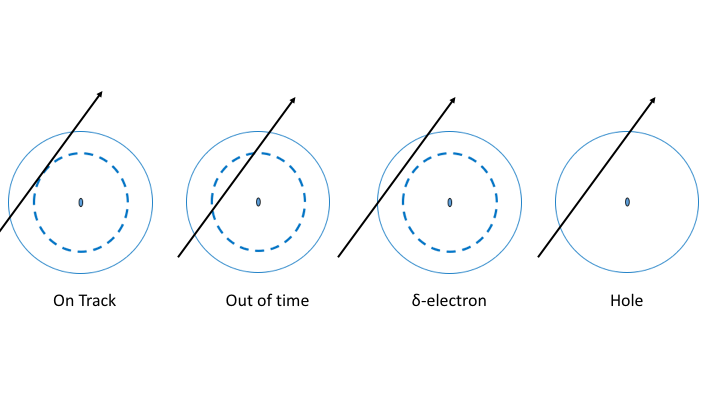
\includegraphics[width=\textwidth]{figures/mstrackMDT.png}
	\caption{Illustration of track fitting in the MS. A track fit to an MDT can be any of 4 cases: track path coincides with drift circle (on track), 
is smaller than drift circle (out of time), is larger than drift circle ($\delta-$electron), and no drift 
circle (hole). Track quality is evaluated by the multiplicity of these cases.}
	\label{fig:mstrackQ}
\end{figure}

\par Full track reconstruction is done by fitting segments, starting from segments farthest 
from the IP and taking into account the bending caused by the 
magnetic field. Each track's $\chi^2$ and number of hits are evaluated and used to 
recursively resolve ambiguities. Finally, the reconstructed tracks are extrapolated to the 
beam-line and their $d_0$ and $z_0$ are extracted. 
    
